\documentclass[11pt,a4paper,twoside,titlepage]{scrartcl}%{scrbook}
\usepackage{a4}

%\usepackage[ngerman]{babel}
%\usepackage{ngerman}
\usepackage[T1]{fontenc}
\usepackage[utf8]{inputenc}

\usepackage{enumerate}
\usepackage{url}
\usepackage{graphicx}
\usepackage{verbatim}
\usepackage[pdfborderstyle={/S/U/W 0},pdfpagelabels,plainpages=false]{hyperref}

% kein einrücken bei paragraphen, stattdessen abstandzeile
\setlength{\parindent}{0pt}
\setlength{\parskip}{1em}

\renewcommand{\textfraction}{0.05}
\renewcommand{\topfraction}{0.95}
\renewcommand{\bottomfraction}{0.95}
\renewcommand{\floatpagefraction}{0.35}
\setcounter{totalnumber}{5}

% die Code-Umgebung einbinden
\usepackage{listings}

% Standard-Layout für die Code-Umgebung (alle Sprachen)
\lstset{%
 	basicstyle=\footnotesize\ttfamily,
	moredelim=[is][\bfseries]{|}{|},
	showspaces=false,
	showtabs=false,
	columns=fixed,
	numbers=left,
	frame=none,
	numberstyle=\tiny,
	breaklines=true,
	showstringspaces=false,
	xleftmargin=1cm,
	tabsize=4
}%

\newcommand{\todo}[1]				{{\em [#1]}\marginpar{{\bf [!!!]}} }
\def\tm{\textsuperscript{\texttrademark}}

\usepackage{color}
\def\red{\textcolor{red}}
\def\blue{\textcolor{blue}}
\def\green{\textcolor{green}}
\def\se{\textcolor{red}}

% hohe penalty für footnote breaks.
\interfootnotelinepenalty=10000

%opening
\title{SpyGlass Manual}
\author{Daniel Bimschas \and Sebastian Ebers \and Dariush Forouher \and Oliver Kleine}
\date{Version 1.0 (\today)}

\pagestyle{headings}
\pagenumbering{roman}

\begin{document}

\maketitle

\tableofcontents

\clearpage
\setcounter{page}{1}
\pagenumbering{arabic}

\section{Introduction}
\label{section:s_introduction}

	\subsection{What is SpyGlass?}
		SpyGlass is an application primarily designed to visualize sensor networks on 
		a screen. It displays a set of sensor nodes at their location on a map, as well 
		as arbitrary data sent by the nodes, e.g. connectivity status between nodes or 
		aggregated data collected by the nodes’ sensors.
	
		The SpyGlass application itself is a framework, designed to be extendable by 
		plugins that visualize arbitrary things. In fact, all visualization and data aggregation
		that is currently done, is done by a set of bundled plugins, each fulfilling a 
		certain functionality. As said before, the primary focus of SpyGlass is the
		visualization of a set of sensor nodes, forming a network. However, SpyGlass can
		also be used in other, nearly arbitrary scenarios, where packet based communication 
		is used. This is because visualization is done based on network packets, 
		which represent statistical, structural or any other arbitrary data, sent by the 
		nodes to the SpyGlass application. Those packets are then dispatched to the 
		various plugins, which in turn, interpret the packet, draw things onto the screen 
		when appropriate and aggregate data contained in the packet. The whole range of visualization 
		opportunities, delivered by the currently bundled plugins, will be explained in 
		this document in the various chapters describing the bundled plug ins.
		
		SpyGlass bases on the requests given by the Institute of Telematics (ITM) of 
		the University of Lübeck and was developed by Daniel Bimschas, Sebastian 
		Ebers, Dariush Forouher and Oliver Kleine in the context of a case study for 
		professional product development.

	\subsection{Installation}
	
		\subsubsection{Prerequisites}
			The SpyGlass application is available in two different versions. One is a plugin 
			for the iShell \footnote{see http://www.coalesenses.com/index.php?page=ishell}
			software, the other is a standalone version. For both versions, a 
			Java Runtime Environment (version 6.0 or newer) is necessary. For the iShell 
			version one needs a platform that is supported by iShell, which is currently 
			Windows and Linux.

			Tested plattforms are:

			\begin{itemize}
			  \item Linux x86
			  \item Linux AMD64
			  \item Windows (32bit)
			  \item Mac OS X with 64bit JRE (experimentally)
			\end{itemize}

		\subsubsection{Build instructions}
		
			The Spyglass project is hosted on SourceForge.net
			(\url{http://sourceforge.net/projects/itm-spyglass}).
			
			You can check out it’s sources with a Subversion client from
			\url{https://itm-spyglass.svn.sourceforge.net/svnroot/itm-spyglass}.

			Spyglass can be used in two ways:

			\begin{itemize}
			  \item{Either as a standalone application or}
			  \item{as a plugin inside the iShell tool.}
			\end{itemize}

			Since Spyglass uses the SWT framework, one has to
			decide at compile-time which platform one wants to use.

			Building Spyglass is very easy. One does not need any external
			libraries besides a working Java SDK and "ant".
			The resulting jar files contain all needed libraries (via the
			One-JAR\tm  boot-mechanism) and are directly executable.

		\subsubsection{Building Spyglass as a standalone application}

			Just run one of

			\begin{verbatim}
			    $ ant standalone-linux
			    $ ant standalone-linux64
			    $ ant standalone-win32
			    $ ant standalone-osx
			\end{verbatim}

			depending on the platform you want to run Spyglass on.

			These commands will build the file \texttt{spyglass-XXX-standalone.jar}, where
			\texttt{XXX} stands for the chosen architecture.
			This jar file includes all necessary dependencies and can be run directly via

			\begin{verbatim}
			    $ java -jar spyglass-XXX-standalone.jar
			\end{verbatim}

		\subsubsection{Building iShell with Spyglass included as a plugin}

			To build iShell with SpyGlass plugin one needs to run one of the commands

			\begin{verbatim}
				$ ant ishell-linux
				$ ant ishell-linux64
				$ ant ishell-win32
				$ ant ishell-osx
			\end{verbatim}

			depending on the platform one wants to use.

			These commands will build the file \texttt{ishell-XXX-spyglass.jar}, where
			\texttt{XXX} stands for the chosen architecture.
			This jar files includes a version of iShell, the compiled Spyglass source
			and all libraries both applications depend on.

			Similarly, it can be run directly via

			\begin{verbatim}
				$ java -jar ishell-XXX-spyglass.jar
			\end{verbatim}

\section{Using SpyGlass}
	
	\subsection{The application interface}

		As mentioned before, there are two different ways to start SpyGlass. First one 
		can start the standalone application, secondly it is a plugin for iShell. For the 
		latter one must start iShell first and activate the SpyGlass plugin afterwards. 
		All screenshots included in this manual are taken from SpyGlass as an iShell 
		plugin.

		On the first start of SpyGlass with an empty configuration one can see the 
		following things (see figure \ref{pic:spyglass_first_appearance}):
		
		\begin{figure}[htb]
			\begin{center}
				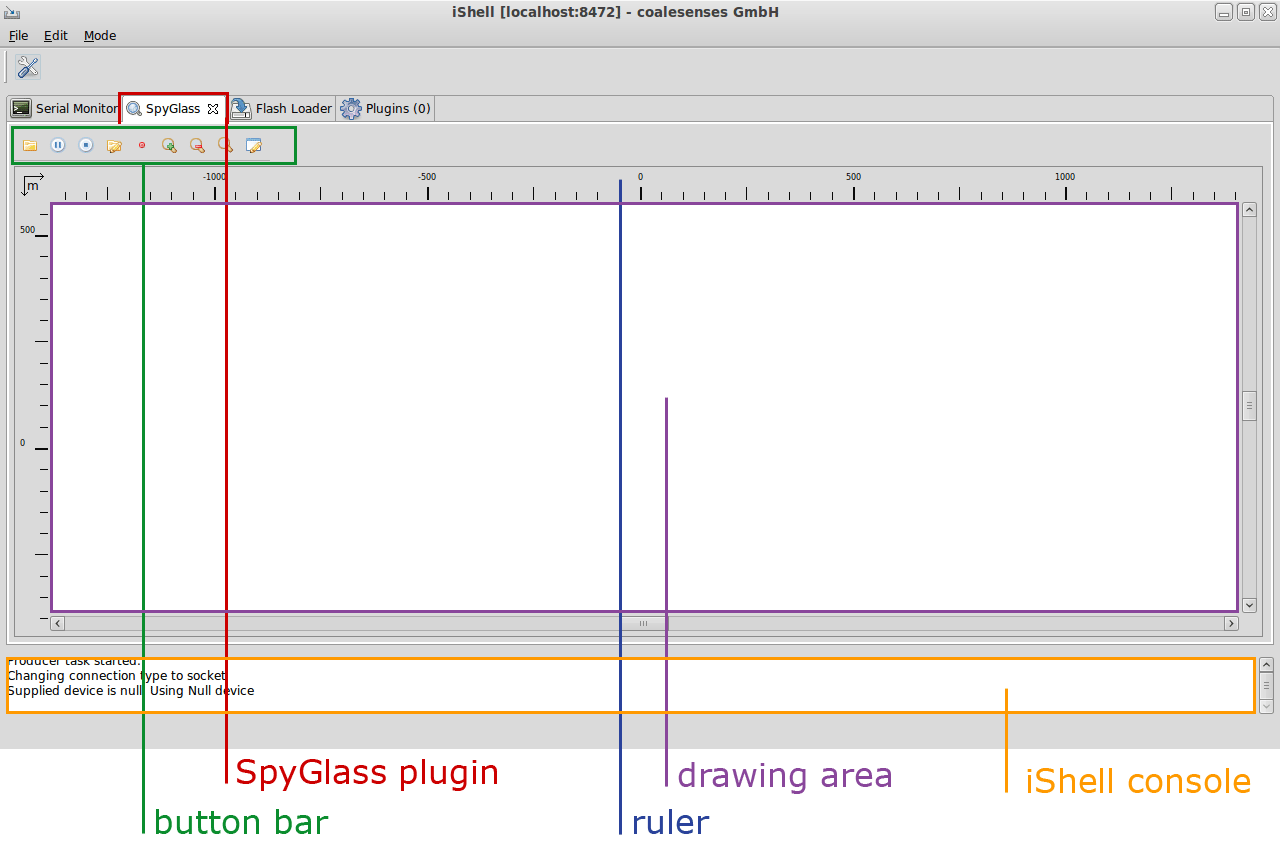
\includegraphics[width=13.2cm]{./pics/spyglass_first_appearance}
				\caption{Empty screen of the SpyGlass plugin for iShell}
				\label{pic:spyglass_first_appearance}
			\end{center}
		\end{figure}
		
		\begin{itemize}
			\item SpyGlass plugin\\
				As iShell contains of many plugins one must explicitly click on the tab for 
				the SpyGlass plugin to bring SpyGlass to the front.
			\item Button Bar\\
				all functions necessary to control the behaviour of SpyGlass can be found 
				here (check subsection \ref{ssec:buttons_behaviour} for a more detailed description).
			\item Drawing Area\\
				All visualization of the sensor network will take place here. The drawing 
				area shows a section of the whole sensor network. This section can be 
				enlarged by zooming out or downsized by zooming in. To change the 
				section to be shown on the drawing area without changing the zoom level, 
				one can either use the scrollbars on the bottom and on the right side of 
				the drawing area or hold the left mousebutton when the pointer is located 
				on the drawing area and move the mouse to the desired direction.
			\item Ruler\\
				The rulers’ labeling represents the current section of the drawing area 
				with respect to the real coordinates. Thus the labels of the ruler change 
				automatically, whenever the drawing area is either moved or if the zoom 
				level changes.
			\item iShell Console\\
				Logging console of the iShell application. iShell plugins print out log 
				messages to the console during runtime.
		\end{itemize}
		
		\paragraph{Differences in the standalone version}
			
			In the standalone version, all functionalities accessible by buttons in the button
			bar are also accessible via the windows’ menubar. Also, there is no iShell
			console in the standalone version.
			
	\subsection{Buttons and their behavior}
	\label{ssec:buttons_behaviour}

		\begin{figure}[htb]
			\begin{center}
				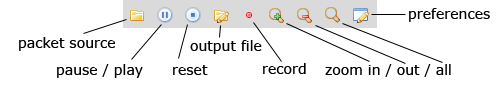
\includegraphics[width=11cm]{./pics/spyglass_buttons}
				\caption{SpyGlass buttons}
				\label{pic:spyglass_buttons}
			\end{center}
		\end{figure}

		In the following all buttons’ functionalities will be explained:
		
		\paragraph{Packet Source}
		  The button opens a dialog to define the current packet source. The source 
		  can either be iShell (through a TCP/IP socket connection) or a file. If 
		  the packet source is iShell, then the packets come from network. The real 
		  packet source (i.e. the packet source where iShell receives packets from)
		  must then be configured by setting the TCP/IP preferences of iShell.
		  
		  \emph{Please note:} In the standalone version of SpyGlass it is only possible to 
		  choose a file as packet source. For more information about how to generate 
		  such a file check the reference for the output file and record buttons.
			
		\paragraph{Pause / Play}
		  Clicking the pause button will stop the SpyGlass application delivering 
		  the sensor nodes’ packets to the various plugins currently active. By this, 
		  the visualization will freeze for the most parts as the plugins don’t receive 
		  new packets. However, some ob jects on the drawing area could disappear 
		  because they time out or they could move to another position for any 
		  reason (e.g. when using a SpringEmbedderNodePositioner, see subsection 
		  \ref{subsection:sep}). Also, plugins doing statistical calculations including
		  timing information, such as packets per second, will therefore display falsified
		  information during the time SpyGlass is paused.
		  
		  All new packets coming in during the time SpyGlass is paused, are queued. 
		  They are delivered sequentially after the play button has been clicked. The 
		  pause button toggles to a play button when it was clicked and vice versa.
				
		\paragraph{Reset}
		  Clicking the reset button will cause all active SpyGlass plugins to reset.
		  Resetting a plugin means that it forgets all aggregated data and removes
		  all drawings from the drawing area. You could say that, after all plugins
		  are reset, the application displays the same information as it displays
		  directly after startup. However, the configuration of plugin instances are kept.
				
		\paragraph{Output File / Record}
		  The record button is to start the recording of incoming packets. One must
		  specify a file, where the incoming packets will be written into. The file gets
		  the ending “.rec” and can be used later in both the standalone application
		  and the SpyGlass iShell plugin as a packet source. The record stops if one
		  clicks on the record button again. During the recording time, the button
		  is white. Otherwise it is red.
				
		\paragraph{Zoom In / Out / All}
		  The “+” and “-” buttons with the magnifier are pretty self-explanatory.
		  One zooms in (+) while the other zooms out (-). The third magnifier button
		  zooms exactly to the zoom level that all current network components
		  (nodes) are displayed on the drawing area.
		  
		  Additionally to the buttons, zooming can also be done with the scrollwheel
		  on the mouse, if the pointer is located on the drawing area.
				
		\paragraph{Preferences}
		  The button opens the preferences dialog, where you can configure the
		  SpyGlass application, as well as the spyglass plugin instances. All that is
		  described in detail from chapter 5 on.


\section{SpyGlass packets}

As SpyGlass itself is just an application to display something, it obviously needs a source of data where it gets the information
from what can or must be displayed. This information comes from the so called SpyGlass packets, which are syntactically
well-defined data packets. That means, that they must be formatted according to one of the five packet types described
in chapter \ref{packet_types} ff.

All SpyGlass packets consist of a header and a payload, where the header format is equal for all packet types. A header
must always have a length of exactly 19 bytes and contain the information shown in table \ref{packet_header}. Note, that
the numbering of the bytes of a packet starts with 0.

\begin{table}[htdp]
  \begin{center}
    \begin{tabular}{l|l|l|p{3cm}}
      \textbf{Byte no.} & \textbf{type} & \textbf{content} & \textbf{comment} \\
      \hline
      \hline
      0,1 & uint16 & packet length (header + payload) & \\
      \hline
      2 & uint8 & version & currently fixed to ``2'' \\
      \hline
      3 & uint8 & syntax type &  0 = std \newline
				1 = uint8List \newline
				2 = uInt16List \newline
				3 = Int16List \newline
				4 = uInt32List \newline
				5 = Int64List \newline
				6 = FloatList \newline
				7 = variable \\
      \hline
      4 & uint8 & semantic type & \\
      \hline
      5, 6 & uint16 & sender ID & \\
      \hline
      7, 8, 9, 10 & uint32 & current time in seconds &  \\
      \hline
      11, 12 & uint16 & milliseconds of current time & \\
      \hline
      13, 14 & int16 & x-coordinate of senders position & \\
      \hline
      15, 16 & int16 & y-coordinate of senders position & \\
      \hline
      17, 18 & int16 & z-coordinate of senders position & \\
    \end{tabular}
    \caption{SpyGlass packet header}
    \label{packet_header}
  \end{center}
\end{table}



\subsection{Packet types}
\label{packet_types}

\subsection{Neighborhood-Packet}
\label{subsection:neighborhood_packet}

The payload of a Neighborhood-Packet contains a list of uint16 values which represents a list of node IDs.
Its syntax type is consequently ``uint16List''. The list must neither contain a node ID twice, nor the node
ID of the sender itself. See an overview on the payload in table \ref{neighborhood_packet_payload}.

\begin{table}[htdp]
  \begin{center}
    \begin{tabular}{l|l|l}
      \textbf{Byte no.} & \textbf{content} & \textbf{type} \\
      \hline
      \hline
      19, 20 & node ID & uint16 \\
      \hline
      20, 21 & node ID & uint16 \\
      \hline
      22, 23 & node ID & uint 16 \\
      \hline
      ... & ... & ... \\
    \end{tabular}
    \caption{Payload of a Neighborhood-Packet}
    \label{neighborhood_packet_payload}
  \end{center}
\end{table}

\subsection{Coordinates-List-Packet-2}
\label{subsection:coordinates-list-packet-2}

A Coordinates-List-Packet-2 contains a payload, which consists of a list of 2-dimensional coordinates. Each coordinate is
represented by an int16 value. Thus a 2-dimensional position needs two values and consequently the payload must have a length
of a multiple of four bytes. Obviously, its syntax type is ``int16List''. A tabular overview is given in table
\ref{coordinates_list_packet_2_payload}.

\begin{table}[htdp]
  \begin{center}
    \begin{tabular}{l|l|l}
      \textbf{Byte no.} & \textbf{content} & \textbf{type} \\
      \hline
      \hline
      19, 20 & x-coordinate of position 1 & int16 \\
      \hline
      21, 22 & y-coordinate of position 1 & int16 \\
      \hline
      23, 24 & x-coordinate of position 2 & int16 \\
      \hline
      25, 26 & y-coordinate of position 2 & int16 \\
      \hline
      27, 28 & x-coordinate of position 3 & int16 \\
      \hline
      29, 30 & y-coordinate of position 3 & int16 \\
      \hline
      ... & ... & ... \\
    \end{tabular}
    \caption{Payload of a Coordinates-List-Packet-2-Packet}
    \label{coordinates_list_packet_2_payload}
  \end{center}
\end{table}


\subsection{Coordinates-List-Packet-3}
\label{subsection:coordinates-list-packet-3}

A Coordinates-List-Packet-3 is very similar to a Coordinates-List-2-Packet. The only difference is the dimensionality, because
this packet contains positions with three dimensions instead of 2. As each coordinate is represented by an int16 value and
a 3-dimensional position needs three values, the payload must have a length of a multiple of six bytes. The syntax type is
``int16List''. See table \ref{coordinates_list_packet_3_payload} for further details.

\begin{table}[htdp]
  \begin{center}
    \begin{tabular}{l|l|l}
      \textbf{Byte no.} & \textbf{content} & \textbf{type} \\
      \hline
      \hline
      19, 20 & x-coordinate of position 1 & int16 \\
      \hline
      21, 22 & y-coordinate of position 1 & int16 \\
      \hline
      23, 24 & z-coordinate of position 1 & int16 \\
      \hline
      25, 26 & x-coordinate of position 2 & int16 \\
      \hline
      27, 28 & y-coordinate of position 2 & int16 \\
      \hline
      29, 30 & z-coordinate of position 2 & int16 \\
      \hline
      ... & ... & ... \\
    \end{tabular}
  \end{center}
  \caption{Payload of a Coordinates-List-Packet-3-Packet}
  \label{coordinates_list_packet_3_payload}
\end{table}

\subsection{Trajectory-Packet-2}
\label{subsection:trajectory2d}

The payload of Trajectory-Packet-2 represents the way of an object via several 2-dimensional positions and the time it needs
to come from one position to the next. So the payload contains a list of tuples, where the first two elements of each tuple
represents a position. The third element represents the time in seconds, that the object spends between the position given
before and the next position. Although the syntax type is ``int16List'' and all elements are of type int16, the time
element must not contain negative values.

Since the last position specifies the ending point, the last tuple is incomplete. It contains only the two elements
representing the position. Table \ref{trajectory_packet_2_payload} shows the content of the payload.

\begin{table}[htdp]
 \begin{center}
    \begin{tabular}{l|l|l}
      \textbf{Byte no.} & \textbf{content} & \textbf{type} \\
      \hline
      \hline
      19, 20 & x-coordinate of position 1 & int16 \\
      \hline
      21, 22 & y-coordinate of position 1 & int16 \\
      \hline
      23, 24 & duration of moving between & int16\\
      & position 1 and 2 & \\
      \hline
      25, 26 & x-coordinate of position 2 & int16 \\
      \hline
      27, 28 & y-coordinate of position 2 & int16 \\
      \hline
      29, 30 & duration of moving between & int16 \\
      &  position 2 and 3 & \\
      \hline
      ... & ... & ... \\
      \hline
      19 + 6(n-1), 20 + 6(n-1) & x-coordinate of position n & int16 \\
      \hline
      21 + 6(n-1), 22 + 6(n-1) & y-coordinate of position n & int16 \\
      \hline
    \end{tabular}
    \caption{Payload of a Trajectory-Packet-2-Packet}
    \label{trajectory_packet_2_payload}
  \end{center}
\end{table}

\subsection{Trajectory-Packet-3}
\label{subsection:trajectory3d}

The payload of a Trajectory-Packet-3 is very similar to a Trajectory-Packet-2. The only difference is, that the positions
are not given in 2D but in 3D. Thus each position consists of three coordinates. Between two positions the payload contains
the duration, the objects needs to pass the way from one position to the next.

The syntax type is ``int16List''. The duration value must be given in seconds and must not contain a negative number
even though it is an int16 field. See table \ref{trajectory_packet_3_payload} for more details.

\begin{table}[htdp]
 \begin{center}
    \begin{tabular}{l|l|l}
      \textbf{Byte no.} & \textbf{content} & \textbf{type} \\
      \hline
      \hline
      19, 20 & x-coordinate of position 1 & int16 \\
      \hline
      21, 22 & y-coordinate of position 1 & int16 \\
      \hline
      23, 24 & z-coordinate of position 1 & int16 \\
      \hline
      25, 26 & duration of moving between & int16\\
      & position 1 and 2 & \\
      \hline
      27, 28 & x-coordinate of position 2 & int16 \\
      \hline
      29, 30 & y-coordinate of position 2 & int16 \\
      \hline
      31, 32 & z-coordinate of position 2 & int16 \\
      \hline
      33, 34 & duration of moving between & int16 \\
      &  position 2 and 3 & \\
      \hline
      ... & ... & ... \\
      \hline
      19 + 8(n-1), 20 + 8(n-1) & x-coordinate of position n & int16 \\
      \hline
      21 + 8(n-1), 22 + 8(n-1) & y-coordinate of position n & int16 \\
      \hline
      23 + 8(n-1), 24 + 8(n-1) & z-coordinate of position n & int16 \\
      \hline
    \end{tabular}
    \caption{Payload of a Trajectory-Packet-3-Packet}
    \label{trajectory_packet_3_payload}
  \end{center}
\end{table}

\subsection{Data-Packet}
\label{subsection:datapacket}

A Data-Packets payload contains arbitrary data. Its syntax type is flexible but must be defined in the header of the packet.
The possible syntax types are ``uint8List'', ``uint16List'', int16List``, ''uint32List``, ''int64List`` and ''floatList``.
The length of the payload depends on the syntax type.

\newpage
\section{StringFormatter}
\label{section:stringformatter}

The StringFormatter is a utility which is used by several plugins to write specific information on the screen.
A StringFormatter expression combines arbitrary text with information from SpyGlass-packets. The placeholders
in these expressions define the type and the position of the value in the packet. Such a placeholder always
starts with a \% followed by specific letter, that represents the type of the value. All possible value types
and the corresponding letter are shown in table \ref{table:stringformatter_types}. Afterwards the
offset of the value in the packet must be given to complete the placeholder. If the string should contain
a \%, it must be masked as \%\%. A line break must be masked as \textbackslash n.

\begin{table}[htdp]
  \begin{center}
    \begin{tabular}{l|l}
      \textbf{letter} & \textbf{type}\\
      \hline
      \hline
      u & uint8 (unsigned, 1 byte) \\
      \hline
      v & uint16 (unsigned, 2 bytes) \\
      \hline
      U & uint32 (unsigned, 4 bytes)\\
      \hline
      i & int16 (signed, 2 bytes)\\
      \hline
      f & float (signed, 4 bytes)\\
    \end{tabular}
    \caption{Value types for a StringFormatter expression}
    \label{table:stringformatter_types}
  \end{center}
\end{table}

In a packet a signed 16 bit integer must be provided in two's complement, while a float value must be given conform to norm
IEEE 754 (IEEE Standard for Binary Floating-Point Arithmetic for microprocessor systems (ANSI/IEEE Std 754-1985)).

In the following an example is given. Assume a packet with the following content (encoded in hexadecimal):

\begin{verbatim}
E7.DF.A0.00.00.00.32.C8.88.03.EF.89
\end{verbatim}

Then the StringFormatter expression

\begin{verbatim}
 Temp: %U3 Grad\n Battery: %u9 V
\end{verbatim}

would result into the following String:

\begin{verbatim}
 Temp: 50 Grad
 Battery: 3 V
\end{verbatim}

\newpage
\section{SpyGlass Plugins}
\label{section:plugins}

\subsection{General information about plugins}

Each plugin defines a specific functionality. To use this functionality one must create instances of the plugin.
Some plugins do some background computing (e.g. PositionPacketNodePositioner), while others display something
on the screen (e.g. SimpleNodePainter).

Usually there will be more than one visible instance to be displayed on the screen. Thus, one needs to define a ranking,
which instance should be displayed on top of another. So some content of an instance in the background might be hidden
by content of another instance. This is done in the
Plugin overview of the SpyGlass preference dialog (see \ref{subsection:pluginoverview}).

But there is also another advantage for the existence of this ranking. Some plugins may provide actions, if the user
clicks on an object on the screen, e.g. the NodePainter opens or closes an extended view when the double-clicks on
the node. It is always the topmost plugin instance that can handle those events, that catches the command and indeed
handles the event. Since currently only the NodePainter handles events, this feature is more or less for
future use.

\subsection{SpyGlass preferences dialog}

\subsubsection{General preferences}
\label{section:generalpreferences}

On the page for general preferences (see \ref{pic:generalpreferences}) one must define basic values especially for the
relation between the position that
the nodes send and their position on the screen. The unit of length is the unit that will be displayed on the
preference pages of all plugins where parameters concerning any height or width must be set. It has no semantic effect, since
SpyGlass expects all positions given with the packets in coordinates and this coordinates are generally interpreted unitless.

\begin{figure}[htb]
  \begin{center}
    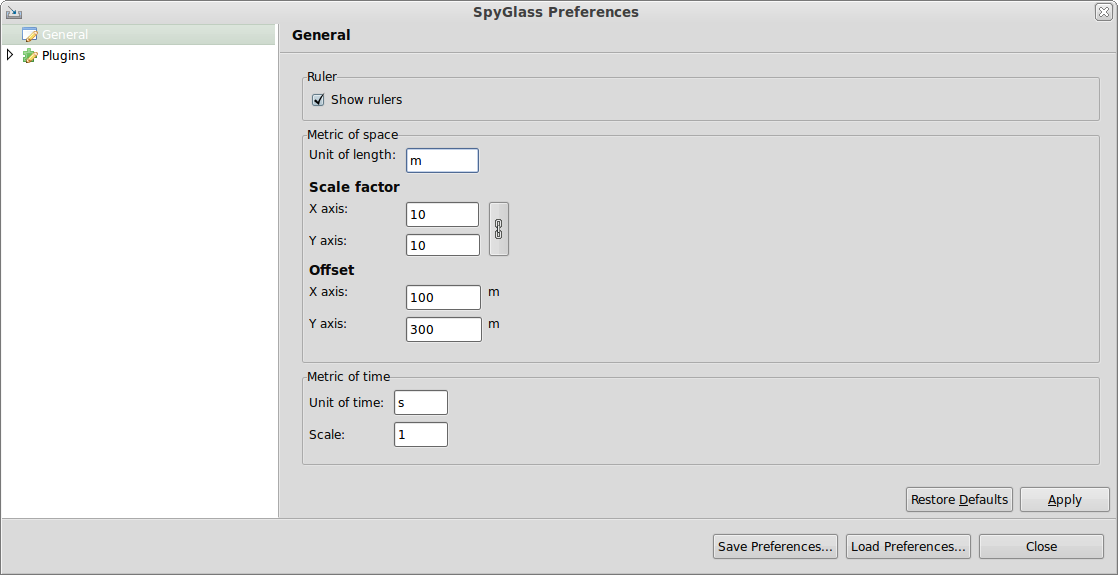
\includegraphics[width=13.2cm]{./pics/general_prefpage}
    \caption{General preferences}
    \label{pic:generalpreferences}
  \end{center}
\end{figure}

The scaling factor defines the scaling of coordinates per dimension. If e.g. an x-coordinate of a position received from
a packet is 5 and the scaling factor of the x-dimension is 20, SpyGlass takes 100 as the real x-coordinate. The scaling
factors of the two dimensions may be defined independently or may also associated to each other by activating the button
with the chain. Then a change of one scaling factor automatically changes the scaling factor of the other dimension to the
same value.

The offset defines the origin of the coordinates. The value of the x-axis is added to all x-coordinates received from a packet.
It is the same for the offset of the y-axis and y-coordinates. If e.g. a packet contains a position (10,10), the x-offset is
set to 50 and the y-offset is set to 80, then SpyGlass takes (60,90) as the real coordinates.

The real coordinates per dimension can be seen in the ruler on the drawing area. The ruler can be set to visible or invisible
on the top of this page.

The button to restore the defaults sets all values to predefined default values. That is ``m'' as metric unit, 1 for the scaling
and 0 for the offset in both dimensions.

The metric of time values are not used anywhere yet. So they are for future use. All values with respect to time have predefined
time units in all current plugins.

\subsubsection{Basic preferences for all plugins}
There is a group of basic preferences which must be configured for all plugin instances. This is the instances name,
at least one semantic type (if the plugin computes packages), the activity status and the visibility.

The name is used to reference to the instance, e.g. in dialog windows. The semantic types define, which packets
will be delivered to this instance. ``-1'' means, that the instance will receive all packets independently from the
semantic type. One can define a comma separated list of semantic types, a range or a combination of both, e.g.
``3-5,8'' is the same as ``3,4,5,8''.

If an instance is not able to compute a packet, because the payload is not
suitable to the plugin, a warning or error window will appear at runtime.

An active plugin instance will receive all packets of the semantic types defined above. Thus, generally spoken
``active'' means, it computes packets. An instance does only display anything, if ``visible'' is set as well.
So, if an instance is active but not visible, it computes the packets in the background.

\subsubsection{Creation of a plugin instance}

Each plugin has a particular page to create instances. On the bottom of all of these pages, one can find the buttons
shown in figure \ref{pic:instance_creation_buttons}.

\begin{figure}[htb]
  \begin{center}
    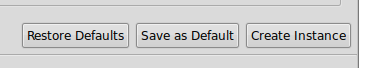
\includegraphics[width=5cm]{./pics/plugin_creation_buttons}
    \caption{Buttons on the page to create a plugin instance}
    \label{pic:instance_creation_buttons}
  \end{center}
\end{figure}

On this page one must configure the instance that shall be created. The configuration can be saved as the new default
configuration. The values of the default configuration will be set on this page whenever it is shown again or the button
``restore default'' is selected. A click on the button ``create instance'' creates an instance of the plugin with the
specified configuration.

If one tries to enter illegal values into the configuration, the changes cannot be applied and a window pops up to tell the
user about the mistake.

\subsection{Change the configuration of an existing instance}

Each plugin instance gets its own entry in the plugin tree of the preference dialog window. Here one can either delete
the instance or change its configuration. If the button ``apply'' is pressed, then the new configuration will be
activated. If one made a mistake while changing the configuration, the old values can be restored with the button
``restore values'' until ``apply'' has been pressed.

\begin{figure}[htb]
  \begin{center}
    
\includegraphics[width=5cm]{./pics/buttons_instance_configuration}
    \caption{Buttons on a plugin instance preference page}
    \label{pic:buttons_instance_configuration}
  \end{center}
\end{figure}

Like on the page for the instance creation, illegal values cannot be applied.


\subsection{Plugin overview}
\label{subsection:pluginoverview}

The plugin overview page presents all plugin instances in a tabular form (see \ref{pic:plugin_instances_overview}).
Here one can do some basic operations
on the instances. At first one can change the order of the plugin. Each instance that is on top of another in this list will
draw its content over all instances contents that should be displayed on the same position on the screen.

\begin{figure}[htb]
  \begin{center}
    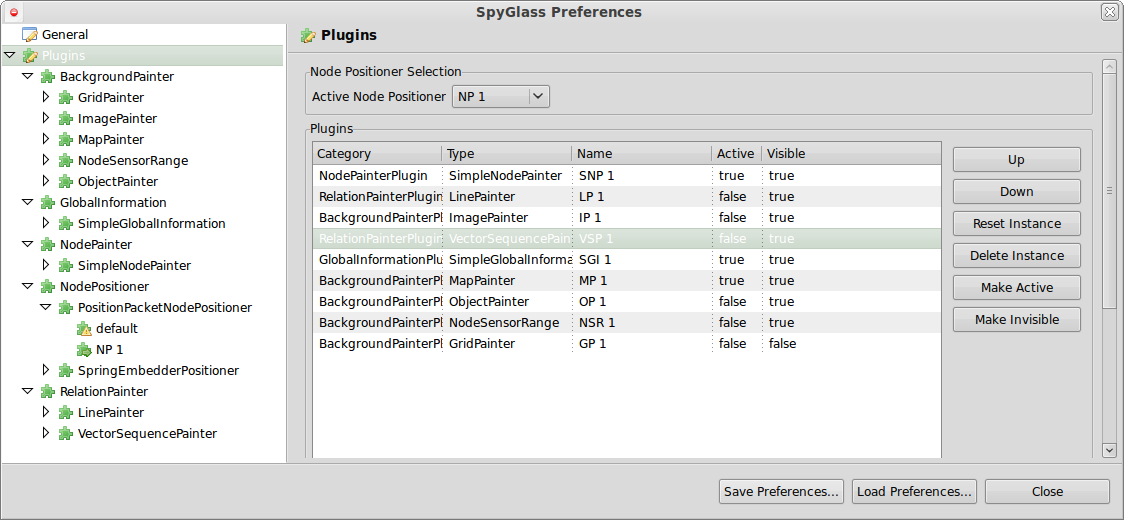
\includegraphics[width=13.2cm]{./pics/plugin_instances_overview}
    \caption{Plugin instance overview}
    \label{pic:plugin_instances_overview}
  \end{center}
\end{figure}

If e.g. an instance SNP of the SimpleNodePainter paints a node as a rectangle and a VectorSequencePainter instance VSP
draws a line that crosses this rectangle, the line is drawn ``behind'' the node (i.e. is invisible) if SNP
is above VSP in the list. Otherwise the line would be drawn above the rectangle. Thus especially BackgroundPainters
should be on the bottom of this list in most cases. To change an
instances position one must simply select the instance and click on ``Up'' or ``Down''.

The button ``Reset instance'' makes the instance to forget all past packets. It has the same effect like deleting the
instance and creating a new one with the same values. ``Delete instance'' deletes the selected instance unrecoverably.

The next two buttons are to change the status of an instance. There labels change automatically on demand.

\newpage
\section{NodePainter}

\subsection{SimpleNodePainter}

The SimpleNodePainter is the main plugin to visualize a sensor network, since it is responsible for the illustration
of the nodes themselves. The configuration page can be seen in figure \ref{pic:snp_preferences}.

Since there are two ways to illustrate a node (``normal'' and ``extended''), one must define which is the default one.
The normal way to display a node is just to write its ID into a rectangle. Color and line width of this rectangle can be configured
as well. The extended illustration shows some additional information which must be defined in the common string formatter
field and the table below. The way how to use the string formatter is described in chapter \ref{section:stringformatter}.

\begin{figure}[htb]
  \begin{center}
    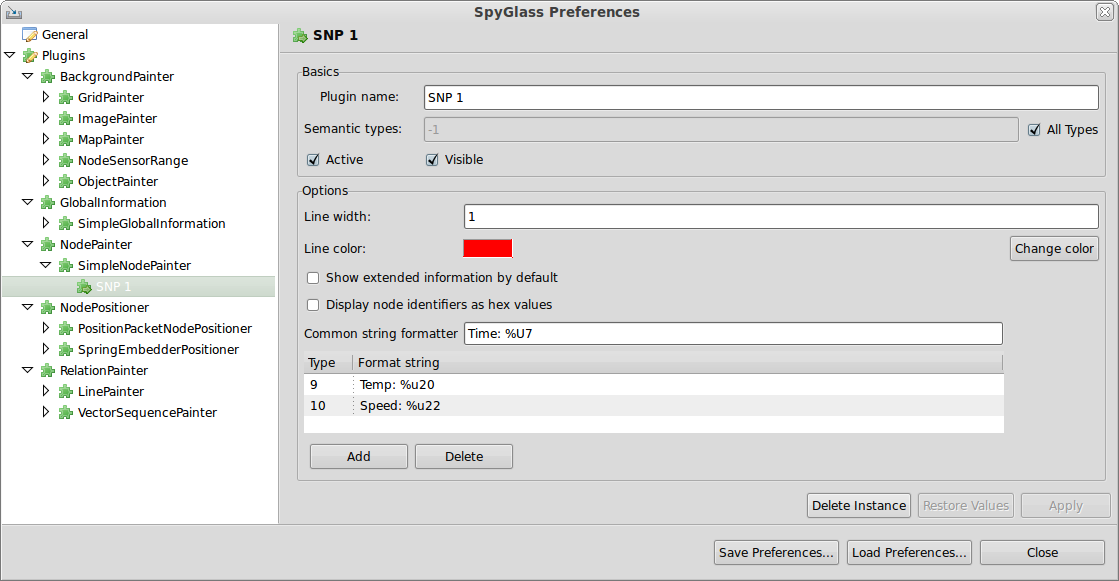
\includegraphics[width=13.2cm]{./pics/simplenodepainter_prefpage}
    \caption{SimpleNodePainter preference dialog}
    \label{pic:snp_preferences}
  \end{center}
\end{figure}

Figure \ref{pic:snp} shows a small network with three nodes. Node 1 is displayed in normal mode, while node 2 and 3 are
in extended mode. As one can see, the common string formatter is responsible for the illustration of the time in the
extended mode while the speed and the temp values are specific to a semantic type.

\begin{figure}[htb]
  \begin{center}
    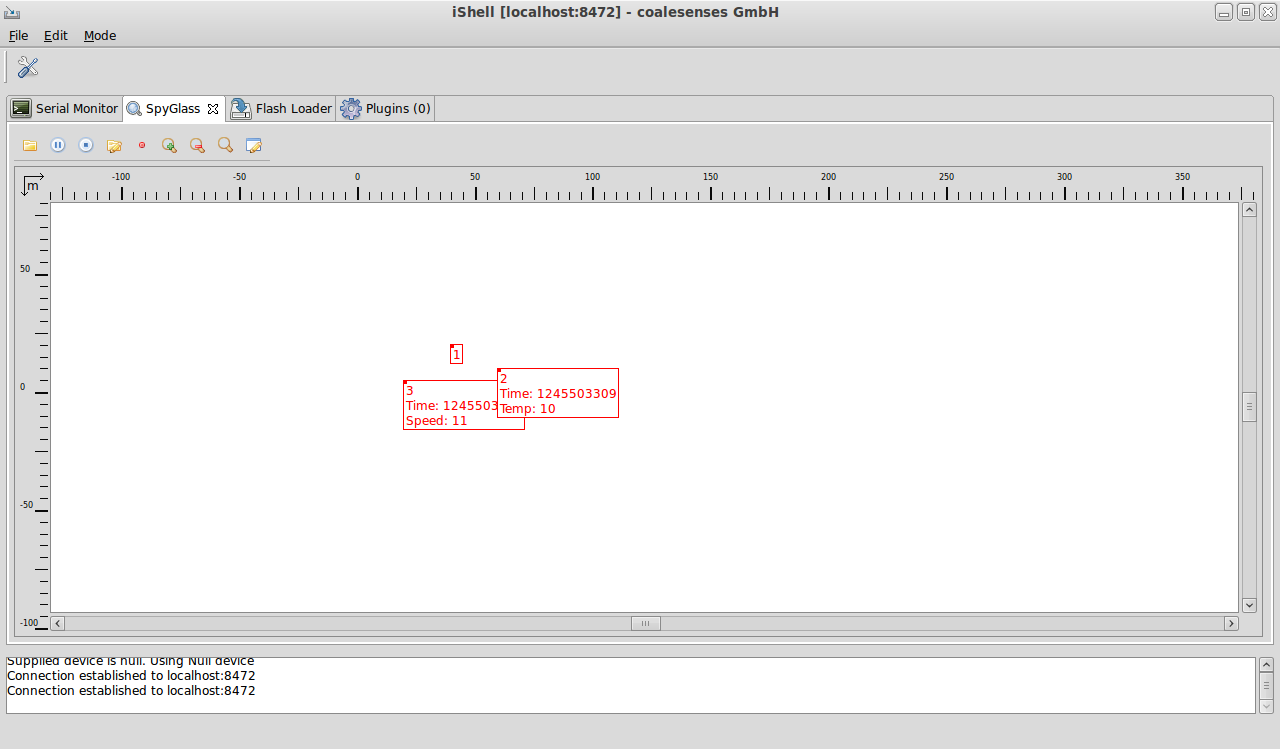
\includegraphics[width=13.2cm]{./pics/simplenodepainter}
    \caption{SimpleNodePainter}
    \label{pic:snp}
  \end{center}
\end{figure}

It is possible to switch between the display modes with a double-click on the node. If a node is in front of another and one
wants to bring the node from the background to the foreground, this can be done with a right-mouse-button-click on
the area of the node in the background. This includes the hidden area of the background node.
In case there is more than one button in the background of another, this click will
bring the node to the foreground, that was the furthest in the background.

The SimpleNodePainter does not need metric information, since it displays the node just at the position that the active
NodePositioner provides. This can be either an instance of the PositionPacketNodePositioner or the SpringEmbedderPositioner.
Both are described in the following chapter.

\newpage
\section{NodePositioner}

A NodePositioner collects and provides the information about the current positions of the nodes in the network. Every incoming
packet will be forwarded to the active NodePositioner instance. This instance grabs the nodes ID, its current position and
the time, when the node sent the packet out of the packets header.

This information is available either until it is overwritten
because the node sent a new packet or until the information times out. The time-out-interval must be set in the preference page
of the instance. On the preference page one can decide, whether the instance is active or not. Since there can only be one
active instance of the NodePositioner plugin, the current instance will be deactivated, when another instance is activated.
The option ``visible'' cannot be set or changed since the plugin instance does not display anything anyway.

There are two types of the NodePositioner plugin which are described in the following chapters \ref{subsection:ppnp} and
\ref{subsection:sep}.

\subsection{PositionPacketNodePositioner}
\label{subsection:ppnp}

An instance of the PositionPacketNodePositioner plugin provides the exact absolute positions for all nodes, who sent
a packet in the past and whose information did not time out yet.

Additionally to the activation status one must define the timeout interval. The interval is set in seconds where 0 means,
that the timeout interval is infinite. Figure \ref{pic:ppnp_preferences} shows the preference dialog
for the PositionPacketNodePositioner

\begin{figure}[htb]
  \begin{center}
    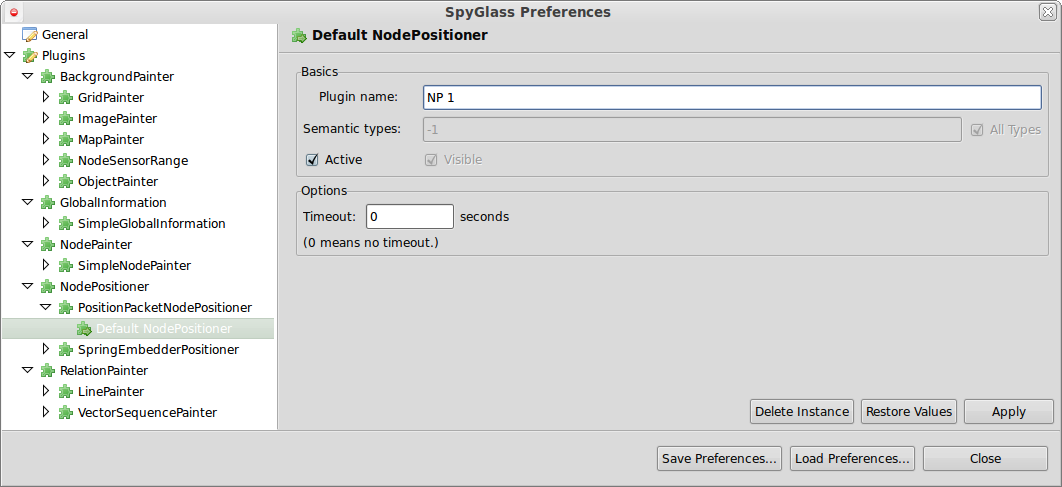
\includegraphics[width=13.2cm]{./pics/positionpacketnodepositioner_prefpage}
    \caption{PositionPacketNodePositioner preference dialog}
    \label{pic:ppnp_preferences}
  \end{center}
\end{figure}

\subsection{SpringEmbedderPositioner}
\label{subsection:sep}

The SpringEmbedderPositioner does not provide absolute positions of the nodes. Instead of absolute positions
a SpringEmbedderPositioner orders the nodes in such a way, that
nodes being in a neighborhood relationship attract each other while the others repulse. For this reason
the positions change dynamically.

All attraction and repulsion forces are being computed for all nodes in the network one after another
once a second. Thus, the positions of all nodes might change permanently, since the distance between the nodes
and thus the forces of attraction and repulsion change in every round.

Additionally to these positions, the SpringEmbedderPositioner stores the current absolute position. So, if an instance of the
PositionPacketNodePositioner plugin becomes active after a SpringEmbedder instance, the new instance will be
initiated with the absolute positions of all known nodes.

If a SpringEmbedderPositioner instance is being activated while another NodePositioner is running, the new
instance will be provided with all nodes and its absolute positions by the old instance. Each of these nodes
gets a random position as a start position for the dynamic computing. The same is valid for new nodes during
the running time of the instance.

There are several values to configure for a SpringEmbedderPositioner instance which is shown in figure
\ref{pic:sep_preferences}. Like a PositionPacketNodePositioner
the SpringEmbedderPositioner has time-to-live for all nodes. If a node does not send a packet for a duration
which is longer than this time-to-live-interval, it will be removed.

\begin{figure}[htb]
  \begin{center}
    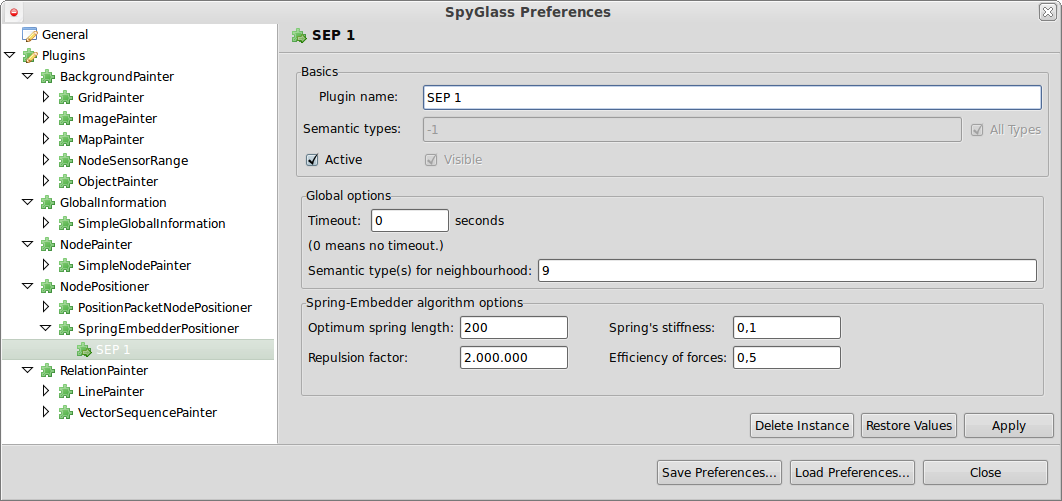
\includegraphics[width=13.2cm]{./pics/springembedderpositioner_prefpage}
    \caption{SpringEmbedderPositioner preference dialog}
    \label{pic:sep_preferences}
  \end{center}
\end{figure}

The most important value is/are the semantic type(s) of the packets, that provide the neighborhood information.
If a node sends such a neighborhood packet (see chapter \ref{subsection:neighborhood_packet}), it will be
attracted by all its neighbors contained in the packets payload. This does not include the reverse, so a sender of the
packet does not attract all its neighbors. A node A is only being attracted by another node B, if node A is contained
in a neighborhood packet sent by node B.

The other configuration values are algorithm specific. The optimum spring length represents the distance, where the
attraction force between to nodes comes into a resting state. The spring stiffness defines, how fast the positions
of the nodes converge to this resting state. The value must be greater than 0 and not greater than 1.

The repulsion factor defines the dimension of repulsion between all nodes, while the efficiency of forces regulates
the speed of the nodes movement. It must be greater than 0 and not greater than 1. Since these values are very
network specific, they should be fitted to the current requirements on demand.

The example given in figure \ref{pic:sep} bases on a network where nodes 1,2 and 3 have a neighborhood relationship
to the node 100 and vice versa. This is also true for 1 and 10-19, 2 and 20-29 and 3 and 30-39. Thus e.g. node 100 has
three neighbors, node 2 has 11 neighbors and node 20 has one neighbor. The figure shows the final resting
position of the nodes. Actually there is no resting position since the algorithm for repositioning the nodes
never comes to an end. But the changes decrease as longer the algorithm runs.

\begin{figure}[htb]
  \begin{center}
    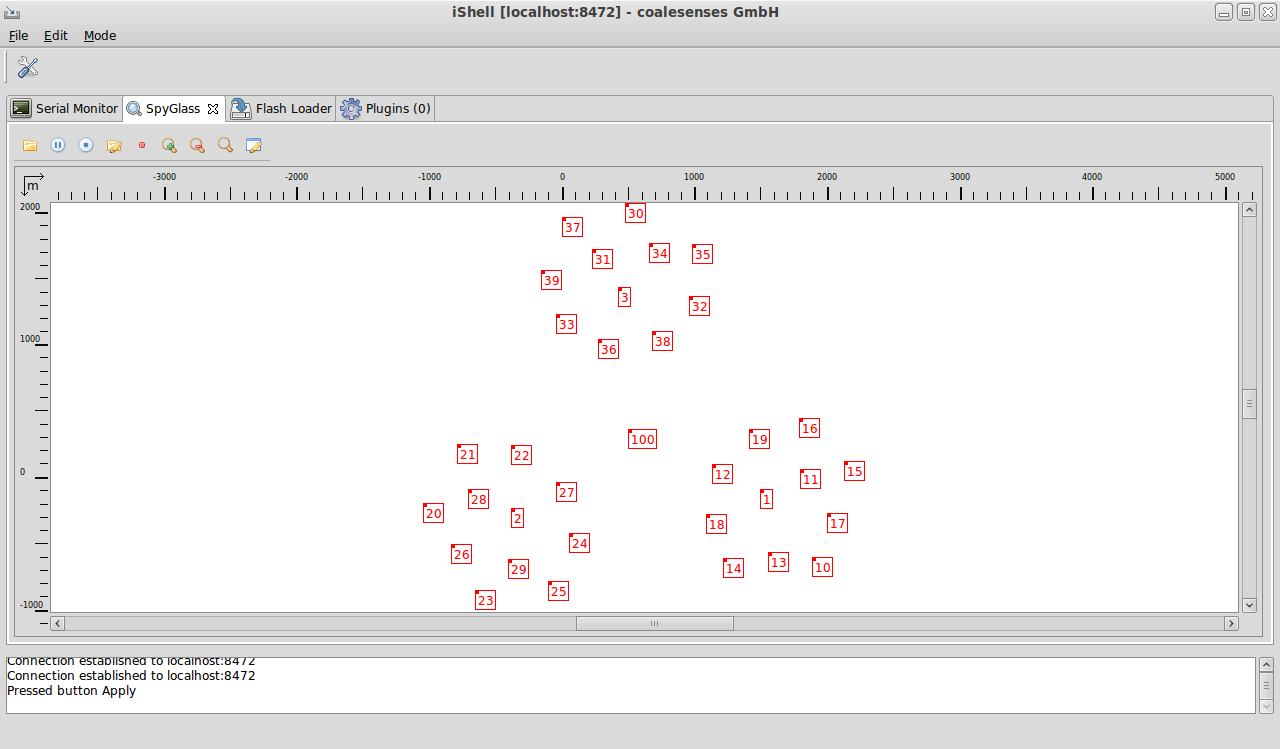
\includegraphics[width=13.2cm]{./pics/springembedderpositioner}
    \caption{NodePainter with active SpringEmbedderPositioner instance}
    \label{pic:sep}
  \end{center}
\end{figure}

Since the PositionPacketNodePositioner provides absolute positions, it provides metrical information.
The SpringEmbedderPositioners positions are not metric. Since some plugins
can only display expedient information if the active NodePositioner instance provides its positions
in such a metric way, all those instances are deactivated automatically when a SpringEmbedderPositioner
instance is getting active. A warning window appears before the automatic deactivation, so the operation
can be stopped. If a plugin needs metrical information or not is described in the appropriate chapter.



\section{RelationPainter}

\subsection{LinePainter}

The LinePainter generally spoken draws a line between two nodes. The LinePainter needs DataPackets containing a uint16 value
at the beginning. This uint16 value defines the neighbor where the line must be drawn to. All following payload starting
at byte 22 (respectively offset 21) of the packet is arbitrary data and can be displayed using
StringFormatter expressions.

The time to live defines how many seconds a line will be displayed. If the time to live is set to 0, the line will
never be removed.

Figure \ref{pic:lp_preferences} shows an example configuration while figure \ref{pic:lp} shows the result of this
configuration.

\begin{figure}[htb]
  \begin{center}
    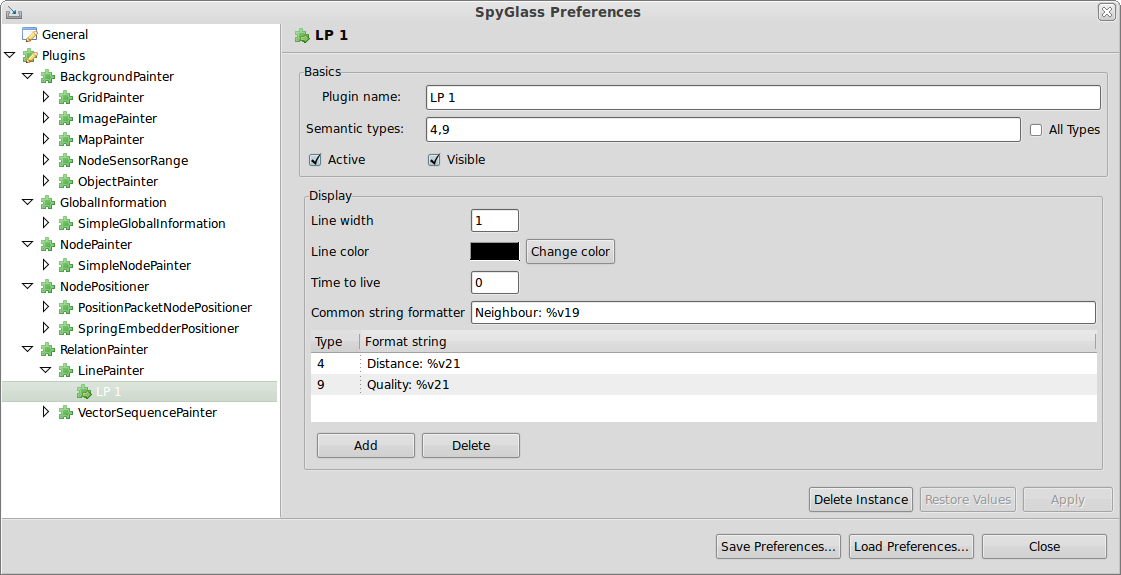
\includegraphics[width=13.2cm]{./pics/linepainter_prefpage}
    \caption{LinePainter preference dialog}
    \label{pic:lp_preferences}
  \end{center}
\end{figure}

As one can see, the strings generated by the StringFormatter expressions are being displayed next to the
sender and above the line between the sender and its neighbor.

\begin{figure}[htb]
  \begin{center}
    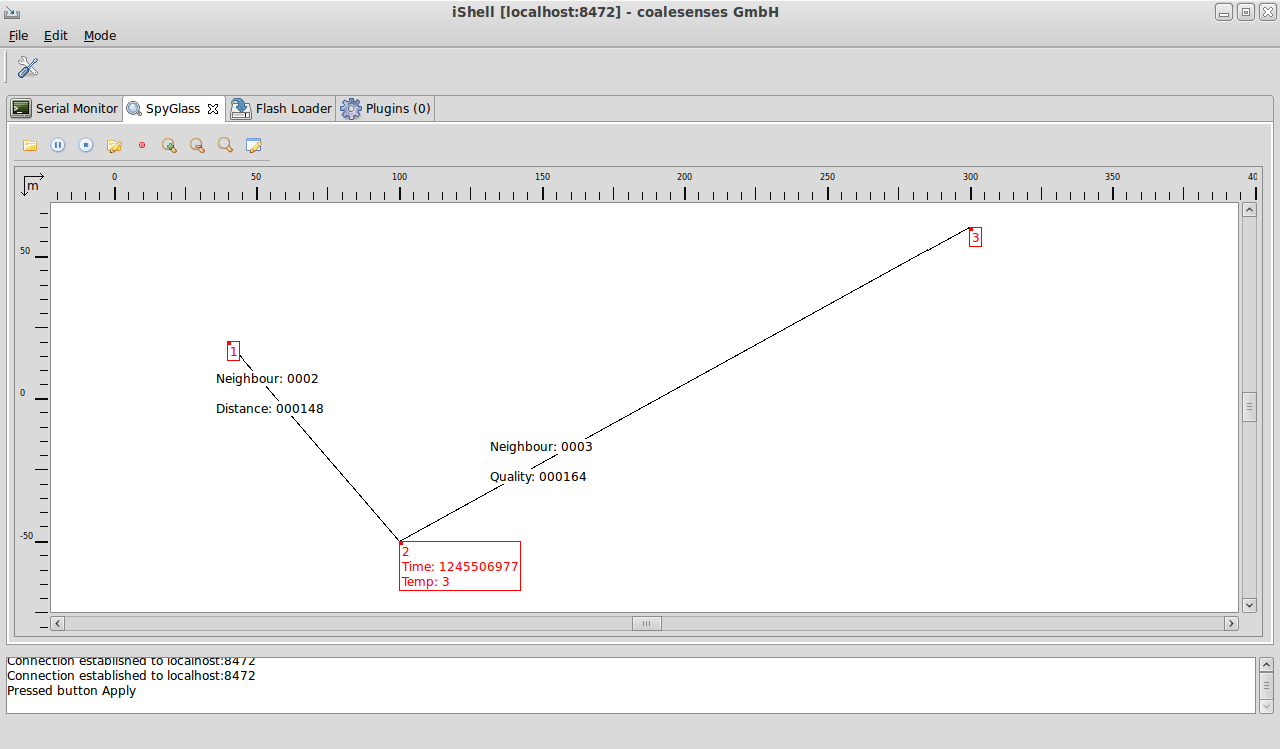
\includegraphics[width=13.2cm]{./pics/linepainter}
    \caption{LinePainter}
    \label{pic:lp}
  \end{center}
\end{figure}

The LinePainter does not need metric positions. It simply draws a line between two nodes.

\subsection{VectorSequencePainter}

A VectorSequencePainter instance draws a sequence of lines. These lines are completely independent from
node positions but could be drawn between arbitrary points. The starting point, edges and endpoint are given
as coordinates via the payload of a Coordinates-List-Packet-2 (see \ref{subsection:coordinates-list-packet-2}) or
a Coordinates-List-Packet-3 (see \ref{subsection:coordinates-list-packet-3}).

This dimensionality of the semantic types, the instance is registered for, must be configured in the preference page
which is shown in figure \ref{pic:vsp_preferences}. All of these semantic types for an instance must have
the same dimensionality. Anyway, in case of 3D, the third dimension will be ignored for the illustration.

All other values in the preference page are pretty self-explanatory.

\begin{figure}[htb]
  \begin{center}
    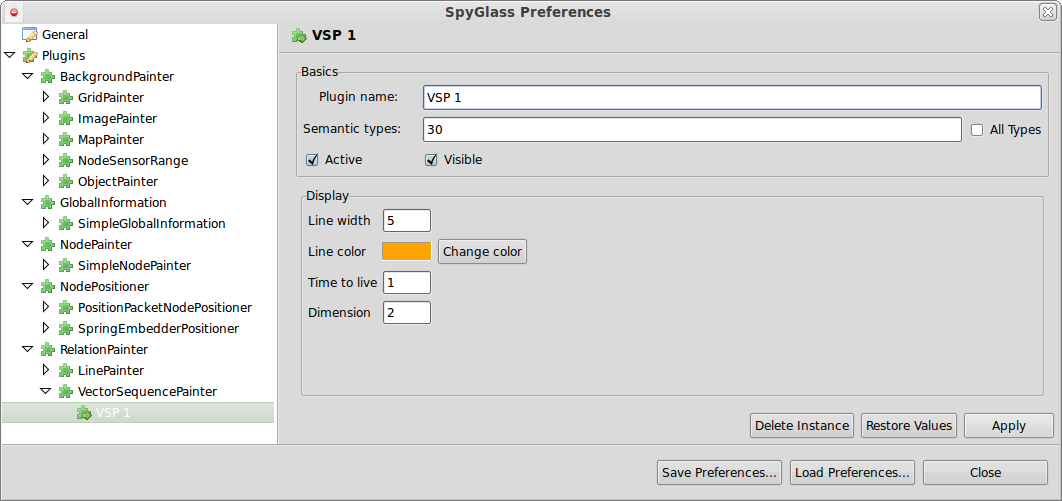
\includegraphics[width=13.2cm]{./pics/vectorsequencepainter_prefpage}
    \caption{VectorSequencePainter preference dialog}
    \label{pic:vsp_preferences}
  \end{center}
\end{figure}

As one can see in picture \ref{pic:vsp}, the position of the lines is completely independent from the position of the
sending node. In this example the data for the line sequence was sent by node 150.

\begin{figure}[htb]
  \begin{center}
    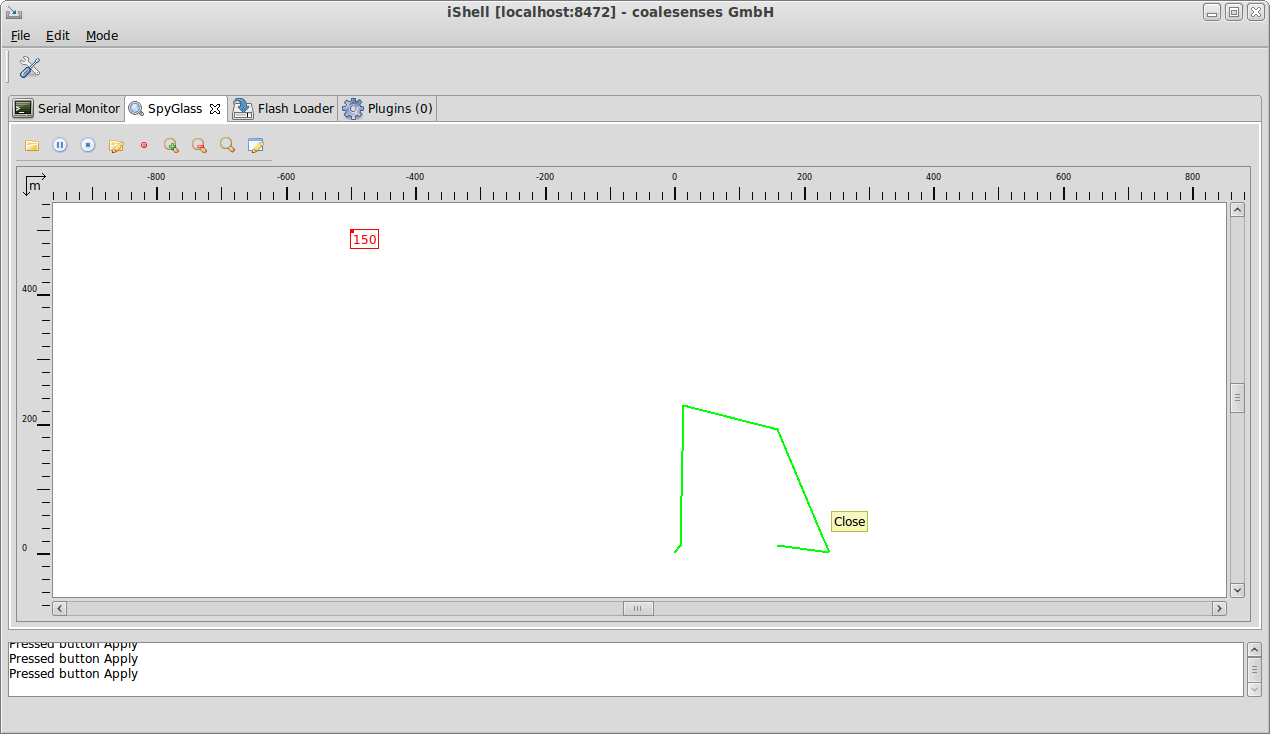
\includegraphics[width=13.2cm]{./pics/vectorsequencepainter}
    \caption{VectorSequencePainter preference dialog}
    \label{pic:vsp}
  \end{center}
\end{figure}

The VectorSequencePainter supports metric, since the starting and ending points of the lines are
given in coordinates with respect to the actual positions in the real world. An instance of the VectorSequencePainter can not
be active while a SpringEmbedderPositioner instance is active as well. Thus it will be deactivated automatically when a
SpringEmbedderPositioner instance is getting active.

\newpage
\section{BackgroundPainter}

\subsection{GridPainter}

An instance of the GridPainter plugin draws a grid with the configured dimensions onto the screen.
One can configure the number of rows and columns independently or associate one to the other with a click
on the button with the chain. If they are associated, then both will have the same value automatically.

It is the same with the width and the height of a grid element. The preference page for an instance of the GridPainter
plugin is shown in figure \ref{pic:gp_preferences}. Since a GridPainter instance does not compute any packets, no semantic type
can be set. To make the grid visible, both active and visible must be set. If one of those is not set, the
is not being displayed.

\begin{figure}[htb]
  \begin{center}
    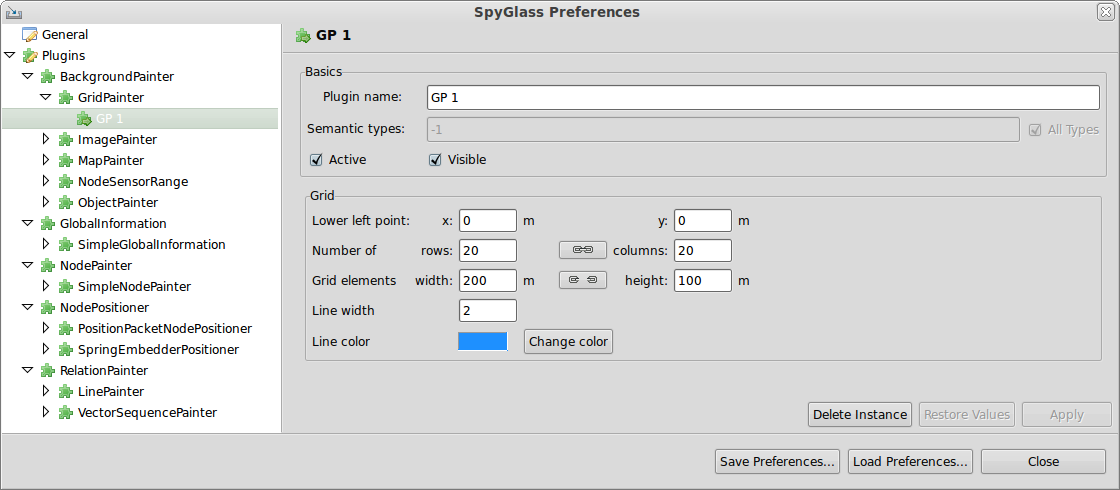
\includegraphics[width=13.2cm]{./pics/gridpainter_prefpage}
    \caption{GridPainter preference dialog}
    \label{pic:gp_preferences}
  \end{center}
\end{figure}

The grid corresponding to the configuration above can be seen in figure \ref{pic:gp}.

\begin{figure}[htb]
  \begin{center}
    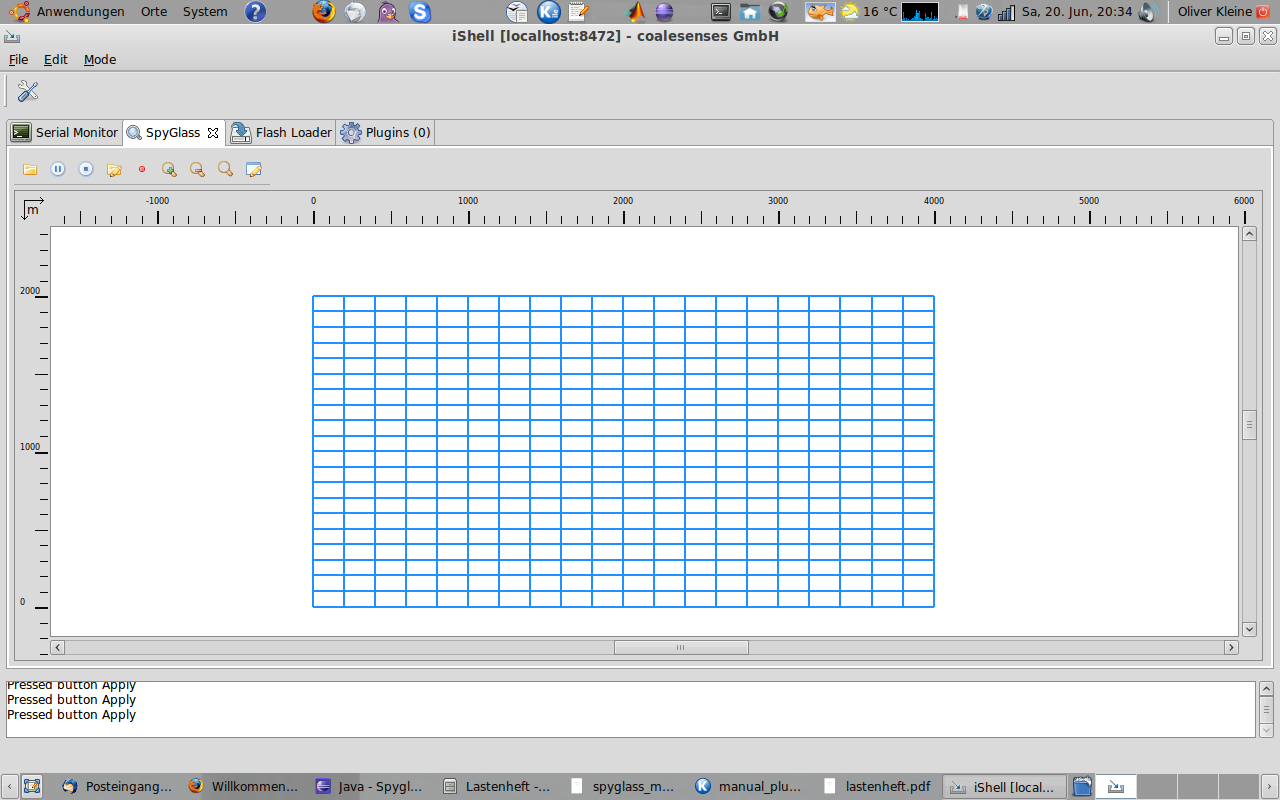
\includegraphics[width=13.2cm]{./pics/gridpainter}
    \caption{GridPainter}
    \label{pic:gp}
  \end{center}
\end{figure}

A GridPainter instance does not support metric. It simply draws a grid at the specified position and the with
the specified size on the drawing area. Thus an instance can be active independently from the type of the
active NodePositioner. If a SpringEmbedderPositioner instance is active, one must ignore the metric units
on the preference page.

\subsection{ImagePainter}

The ImagePainter is to draw an image on the background. This might be an arbitrary image from the local file system.
Supported images types are ``jpg'', ``gif'' and ``png''. See the preference page in figure \ref{pic:ip_preferences}.

The position is set by setting the lower left point in absolute coordinates. The image can be resized either
independently per dimension or with keeping the proportions automatically when changing the value for one dimension.

\begin{figure}[htb]
  \begin{center}
    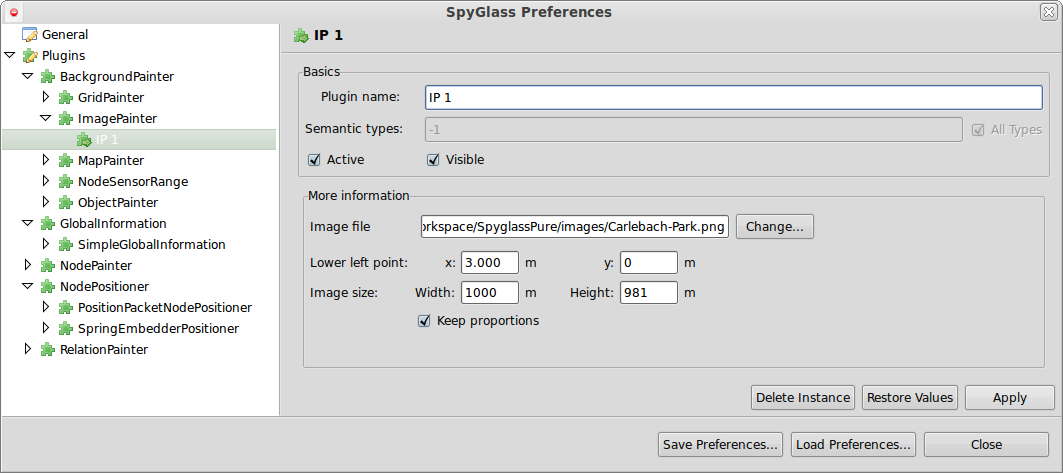
\includegraphics[width=13.2cm]{./pics/imagepainter_prefpage}
    \caption{ImagePainter preference dialog}
    \label{pic:ip_preferences}
  \end{center}
\end{figure}

The ImagePainter does not support metric. It just draws the specified image at the specified position with the specified
size. If a SpringEmbedderPositioner instance is active, one must ignore the metric units
on the preference page.

\subsection{MapPainter}

A MapPainter instance draws a map on the specified sector of the drawing area. This sector must be defined by
setting its lower left point, and its horizontal and vertical comprehensiveness on the preference page (see
\ref{pic:mp_preferences}). The granularity defines the resolution of the map, i.e. the number of independently
computed values (rectangles on the map). The two parameters per dimension for comprehensiveness and resolution can be associated to
each other, i.e. set to the same value automatically, by using the appropriate button with the chain.

\begin{figure}[htb]
  \begin{center}
    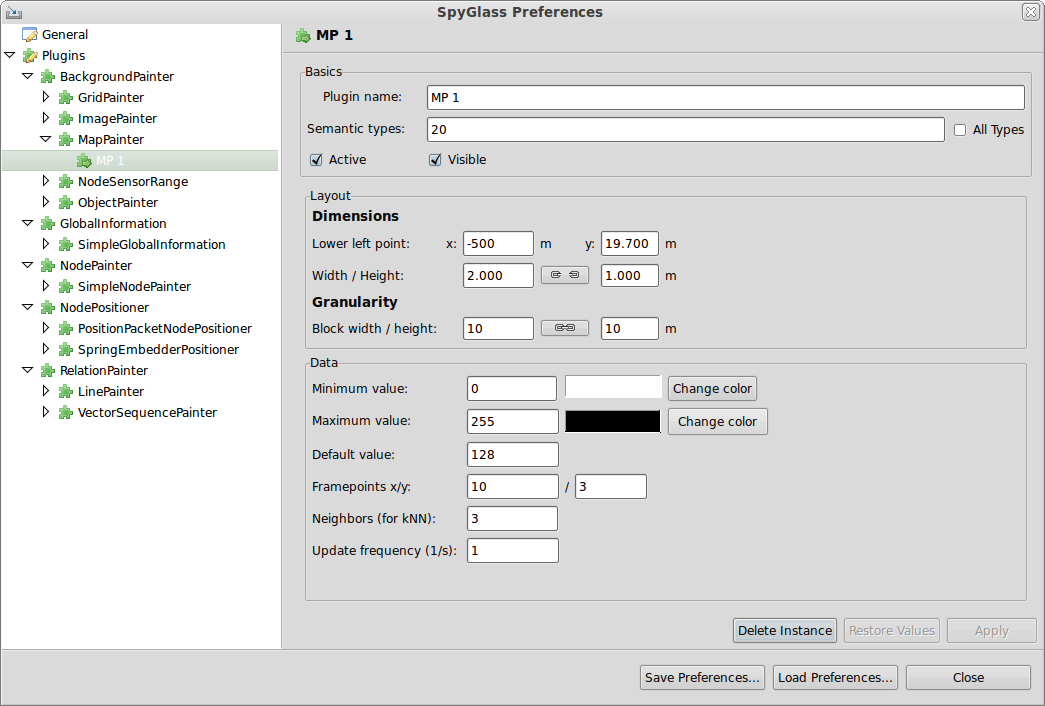
\includegraphics[width=13.2cm]{./pics/mappainter_prefpage}
    \caption{MapPainter preference dialog}
    \label{pic:mp_preferences}
  \end{center}
\end{figure}

The other parameters define the range of data, that is contained in the packets payload. Concerning this
payload, two things must be clarified at the beginning. The MapPainter always uses only the first element of the
payload. If the payload contains for example an int16List, only the first two bytes of the payload are read
and used as an int16 value. The rest of the payload will be ignored. The other thing is, that generally all
packets from nodes, whose position is outside of the maps area will be ignored as well.

The MapPainter associates a color with all possible values. If a value is less than the minimum value from the
preference page it gets the same color as the minimum value. It is the same with values grater than the maximum
value from the preference page. They will be associated with the same color as the maximum value. All values
in between will be associated with a mixed color between the defined colors for minimum and maximum value.

Assume the maximum value is associated with black and the minimum value is associated with white. Then a
value close to but lower than the maximum value will be associated with a dark grey, while a value close to
but higher than the minimum value will be associated with a bright grey.

For each rectangle of the map, the appropriate value is computed by identifying the k nearest neighbors,
i.e. the k nearest positions, where a measured value is known and calculate the mean of these k values.

Each map has frame points. Frame points are invisible points on the maps border, that behave like nodes with
a fixed position and measured data. The positions of the frame points are uniformly distributed on the frame, thus
per dimension the distance between neighbored frame points is equal. Each frame point provides the
default value. The update frequency defines how often the map is being recomputed per second. As the algorithm
to recalculate all the values is computational expensive, the actual update frequency could be slower than the
configured.

Figure \ref{pic:mp} shows an example for a MapPainter instance together with an active and visible SimpleNodePainter
instance. So one can see, where the nodes are located in the maps sector.

\begin{figure}[htb]
  \begin{center}
    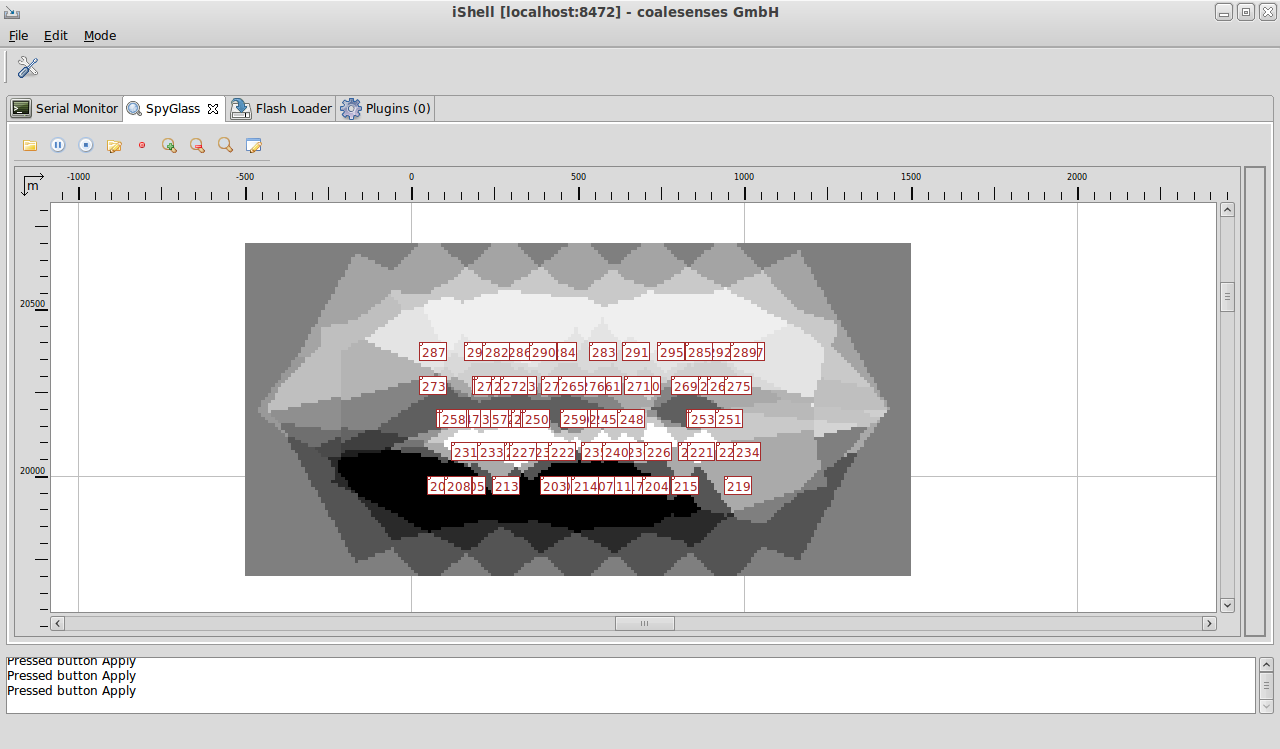
\includegraphics[width=13.2cm]{./pics/mappainter}
    \caption{MapPainter}
    \label{pic:mp}
  \end{center}
\end{figure}

The MapPainter supports metric, since the whole map bases on the distance of the nodes in the real world. Thus an
instance can not be active while a SpringEmbedderPositioner instance is active, too.

\subsection{NodeSensorRange}

An instance of the NodeSensorRange plugin illustrates the area next to the node, that can be covered by a sensor.
One can define many values for a NodeSensorRange instance. The preference page can be seen in figure \ref{pic:nsr_preferences}.

In addition to the usual graphical parameters (line width, color, etc.) one must define the form. Possible
options are ``Circle'', ``Rectangle'' and ``Cone''.
The reference point for the illustration of the sensor range is the position of the node, i.e. the radius
of a circle starts here and the center of a rectangle is here as well. The edge with the acute angle of a the
cone is also located at this position.

\begin{figure}[htb]
  \begin{center}
    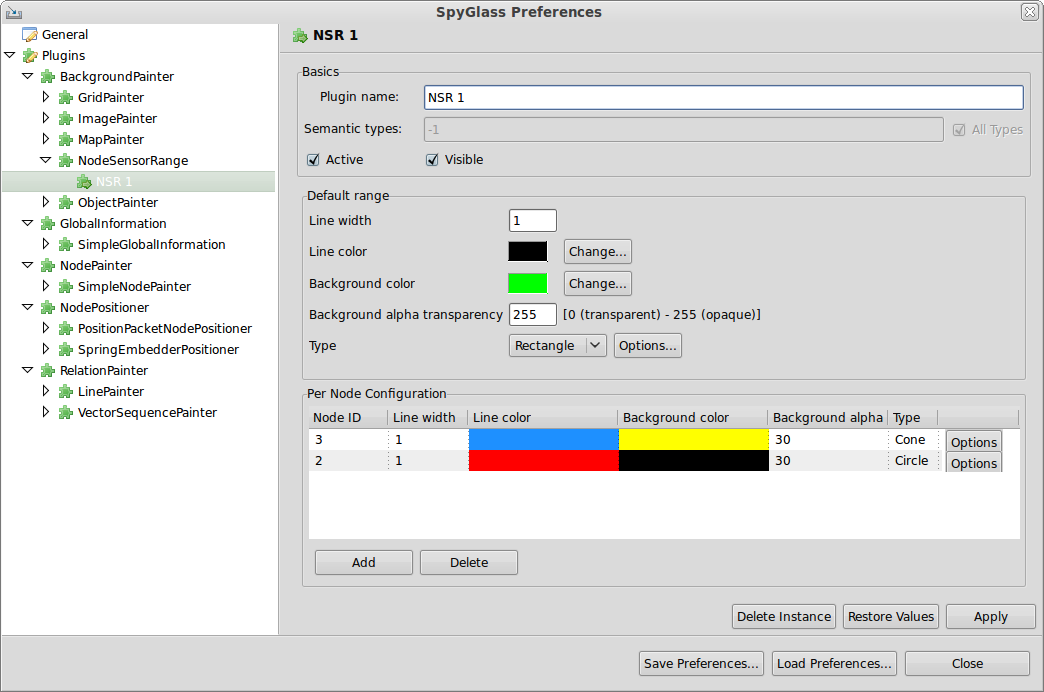
\includegraphics[width=13.2cm]{./pics/nodesensorrange_prefpage}
    \caption{NodeSensorRange preference dialog}
    \label{pic:nsr_preferences}
  \end{center}
\end{figure}

One must define a default range, which will be displayed for all nodes that fo not have a specific configuration in
the table below. The specific configuration for the type of the range can be opened by clicking on the options button
next to the selection field for the type.

The only options for a circle range is the radius. It is given with respect to the generally defined metric unit.
A rectangle needs three parameters. The width and the height that must be defined with respect to the generally
defined metric unit as well. The orientation value defines the angle in degrees how far the rectangle is
turned to the right. A cone has three specific parameters, too. The first parameter is the length, e.g. the
radius of the imaginary circle around the node, where the cone is a part of. Like for rectangles, the orientation
defines the angel in degrees how far the cone is turned to the right. If the orientation angle is 0, the right
edge of the cone is parallel to the x-axis. The view angle defines how wide the range is
in degrees, i.e. a half circle would be 180 degrees.

See the illustration of an example instance of the NodeSensorRange plugin in figure \ref{pic:nsr}.

\begin{figure}[htb]
  \begin{center}
    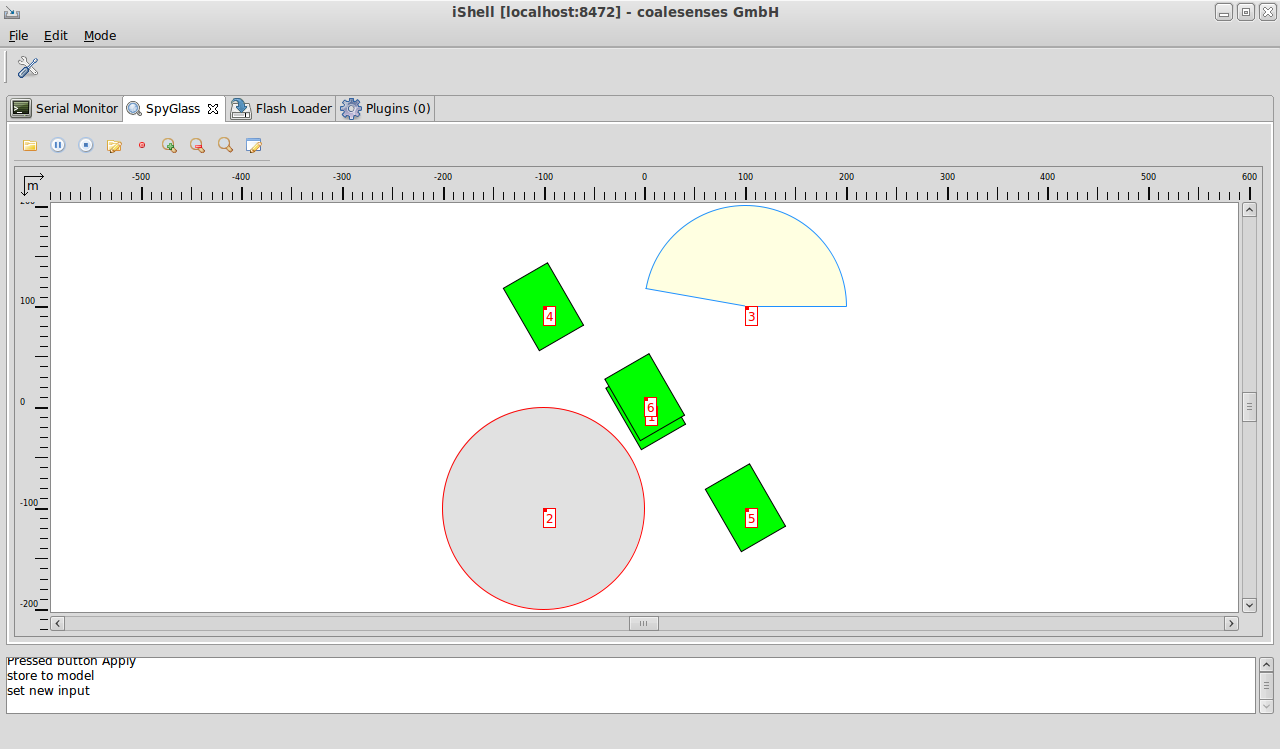
\includegraphics[width=13.2cm]{./pics/nodesensorrange}
    \caption{NodeSensorRange}
    \label{pic:nsr}
  \end{center}
\end{figure}

The NodeSensorRange plugin does not support metric. Thus it can be active together with an active SpringEmbedderPositioner
instance. In case of an active SpringEmbedder, the range information is more informal and not absolute.

\subsection{ObjectPainter}

An ObjectPainter instance draws a moving object on the drawing area. The object to be moved on the screen must be
defined in the field ``image file'' on the preference page (see \ref{pic:op_preferences}).

\begin{figure}[htb]
  \begin{center}
    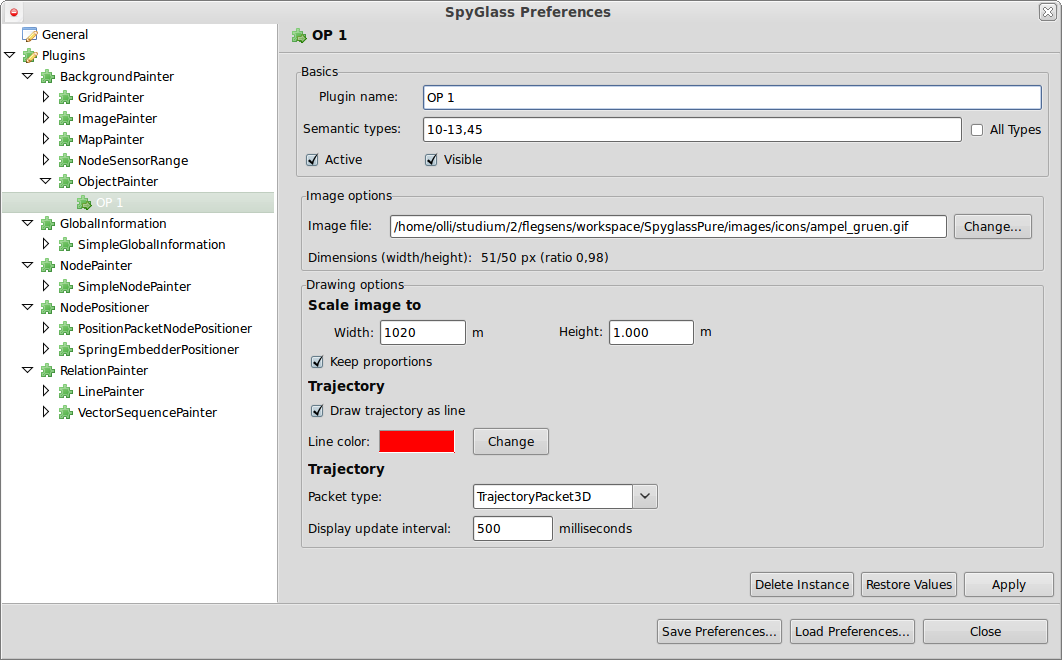
\includegraphics[width=13.2cm]{./pics/objectpainter_prefpage}
    \caption{ObjectPainter preference dialog}
    \label{pic:op_preferences}
  \end{center}
\end{figure}

The drawing options must be set below. At first one can resize the image either with keeping the proportions or by
setting width and height independently. The trajectory is the way the object takes on the screen. This way
can be drawn on the screen with the specified color.

The trajectory is given by the payload of a Trajectory-Packet. This can either contain 2D or 3D coordinates discribing
the way of the object. The packets are explained in the chapters \ref{subsection:trajectory2d} and
\ref{subsection:trajectory3d}. All semantic types the plugin instance is registered for, must be of the same type.
To mix both trajectory types in one network, one must define at least two ObjectPainter instances. Anyway in case of
3D, the third dimension is ignored for illustration.

The last parameter is the update interval. As smaller this interval is, the more
often the plugins illustration is updated, e.g. the more smooth is the movement of the object.

\begin{figure}[htb]
  \begin{center}
    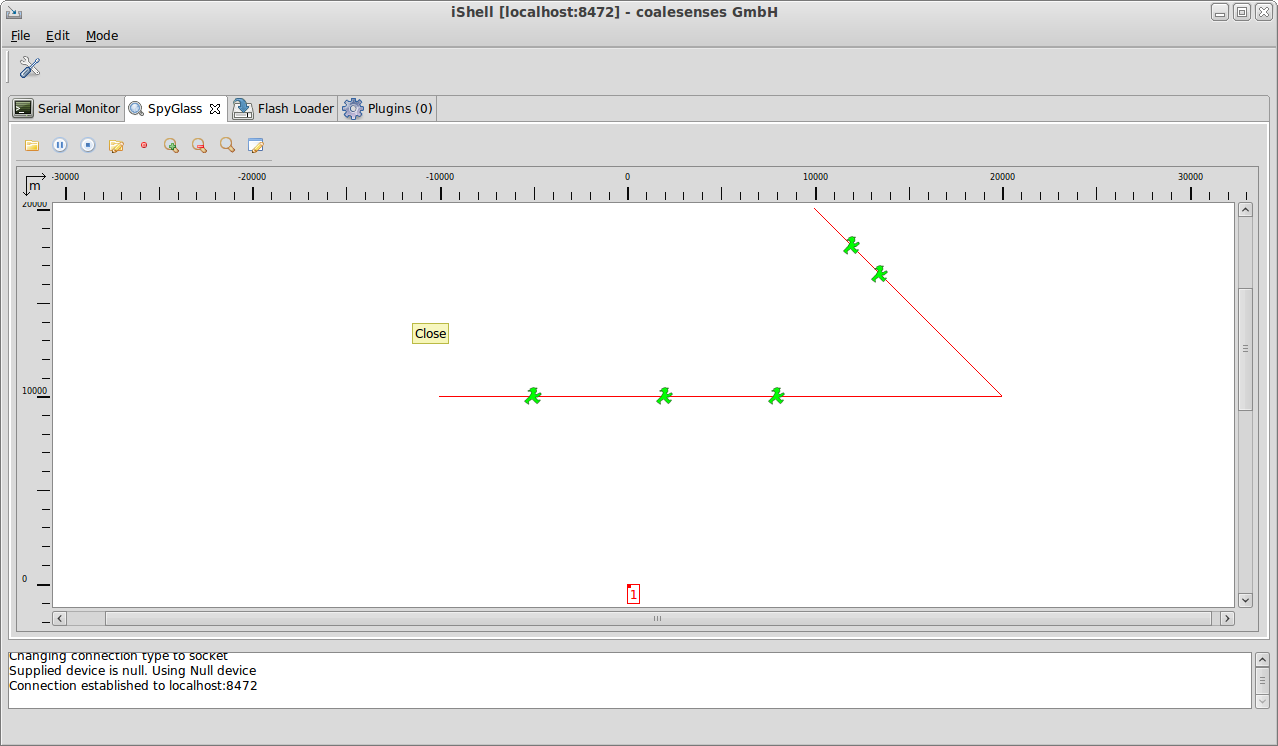
\includegraphics[width=13.2cm]{./pics/objectpainter}
    \caption{ObjectPainter}
    \label{pic:op}
  \end{center}
\end{figure}

The example in figure \ref{pic:op} shows one trajectory but many little man moving on the line. Each of this
little men exists because of one packet, e.g. each packet generates a moving object on the screen. In this
example, all objects take the same way but this is not necessary. An object takes the way, that is defined
by its appropriate tracetory packet.

The plugin supports metric, so an instance can not be active while an instance of the SpringEmbedderPositioner is
active as well.

\newpage
\section{GlobalInformation}

\subsection{SimpleGlobalInformation}
\label{subsection:simpleglobalinformation}

An instance of the SimpleGlobalInformation plugin writes some predefined statistical information on the right
side of the screen.

Each visible instance of a SimpleGlobalInformation plugin displays the number of packets that have been sent
in the network since the instance is active. The next default parameters are the numbers of packets, that have been
received and computed during several periods. PPS means packets per second. The three values afterwards
represent the mean number of packets per second during the last second, the last 30 seconds and the last 60 seconds
This values will always be shown and can not be configured.

The display of some standard information can be directly activated by selecting the appropriate box at the bottom
of the preference page (see \ref{pic:sgi_preferences}). These standard informations are the number of nodes in the
network and the average node degree, i.e. the mean number of neighbors. For this reason there must be one or more semantic
type(s) defined, that contain the neighborhood information (see \ref{subsection:neighborhood_packet}).

\begin{figure}[htb]
  \begin{center}
    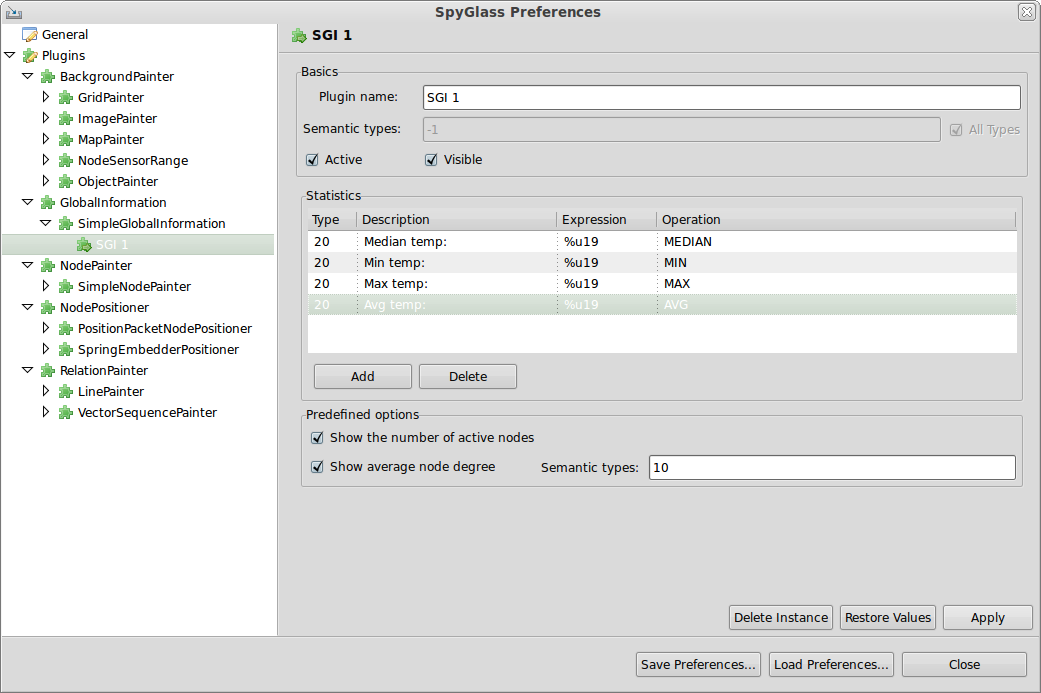
\includegraphics[width=13.2cm]{./pics/simpleglobalinformation_prefpage}
    \caption{SimpleGlobalInformation preference dialog}
    \label{pic:sgi_preferences}
  \end{center}
\end{figure}

The table in the middle of the preference page is for the configuration of some specific statistical information.
Each row in this table belongs to one statistial value. In the example configuration on figure \ref{pic:sgi_preferences}
the packets of semantic type 20 contain a temperature value of type uint8 at the beginning of the packets payload (offset 19).
This data is used to compute some statistics on it. Possible operations are ``sum'', ``minimum'', ``maximum'',
``average'' and ``median''.

Figure \ref{pic:sgi} shows an active instance of the SimpleGlobalInformation plugin together with an active MapPainter.
As the MapPainter draws a map from the temperatures, the SimpleGlobalInformation instance computes some statistics
on the same data.

\begin{figure}[htb]
  \begin{center}
    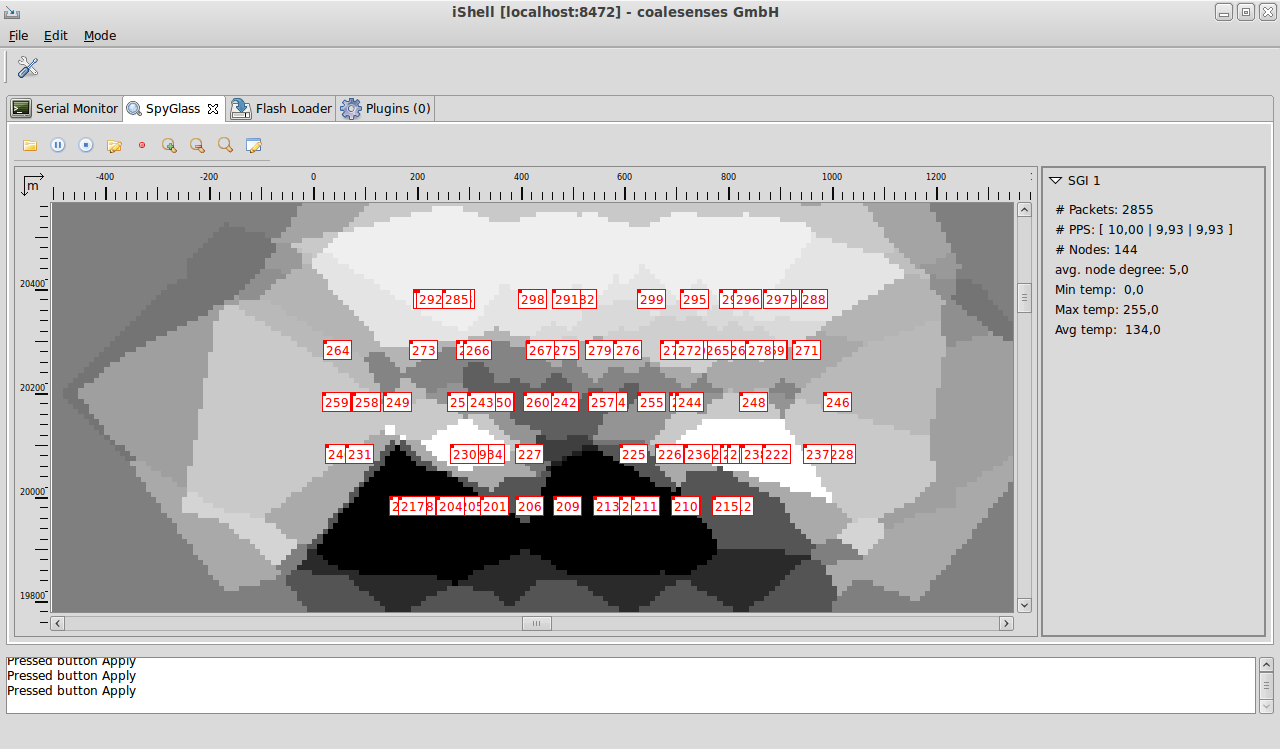
\includegraphics[width=13.2cm]{./pics/simpleglobalinformation}
    \caption{SimpleGlobalInformation}
    \label{pic:sgi}
  \end{center}
\end{figure}



\end{document}
